\documentclass{article}
\usepackage{fontspec}
\usepackage{type1cm}
\usepackage{graphicx}
\usepackage{geometry}
\usepackage[bold-style=ISO]{unicode-math}
\usepackage[heading=true]{ctex}%添加heading=true,使用中文版式
\geometry{a4paper,left=1cm,right=1cm,top=3cm,bottom=3cm}
\usepackage{titlesec} %自定义多级标题格式的宏包
\titleformat{\section}[block]{\Huge\bfseries}{\arabic{section}}{1em}{}[]
\titleformat{\subsection}[block]{\huge\bfseries}{\arabic{section}.\arabic{subsection}}{1em}{}[]
\titleformat{\paragraph}[block]{\LARGE\bfseries}{[\arabic{paragraph}]}{1em}{}[]

\begin{document}
\begin{flushleft}
	\LARGE
	% \qquad 缩进两个字符
	
	\section{公式}

	\subsection{二维邻域}
	以点$P_0(x_0,y_0)$为圆心,$\delta$为半径围成一个圆。圆内所有的点(不包括圆的边)的集合称为$P_0$的$\delta$邻域,记为$U(P_0,\delta)$\\
	
	\subsection{二元函数}
	二元函数$z=f(x,y)$的图像在三维坐标里是曲面\\
	二元函数的可导与连续无关\\
	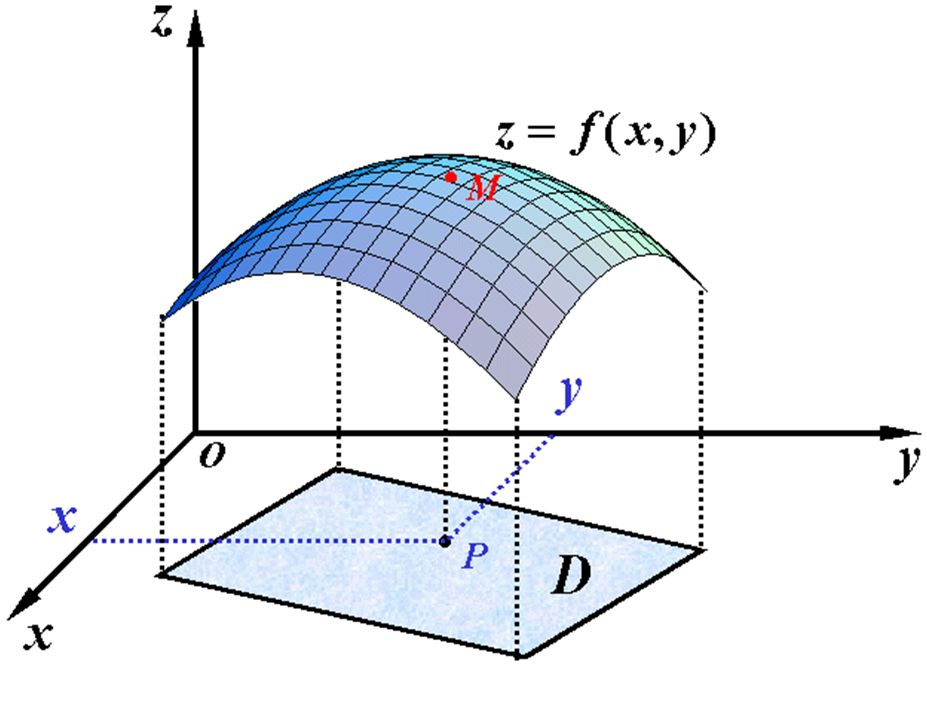
\includegraphics[scale=0.5]{eyhstx.jpg}
	
	\subsection{二元函数的极限}
	$\lim\limits_{\substack{x\to x_0\\ y\to y_0}}f(x,y)=A$\\
	注意:二元函数求极限不能使用洛必达法则和单调有界准则\\
	~\\
	若$\lim\limits_{\substack{x\to x_0\\ y\to y_0}}f(x,y)=f(x_0,y_0)$,则$f(x,y)$在点$(x_0,y_0)$连续\\
	
	\subsection{偏导数}
	\paragraph{偏导数的定义}
	$f_x'(x_0,y_0)=\lim\limits_{x\to x_0}\frac{f(x,y_0)-f(x_0,y_0)}{x-x_0}$\\
	$f_y'(x_0,y_0)=\lim\limits_{y\to y_0}\frac{f(x_0,y)-f(x_0,y_0)}{y-y_0}$\\
	
	\paragraph{求偏导数}
	1、对$x$求偏导:将$y$看作常数后再对$x$求导\\
	2、对$y$求偏导:将$x$看作常数后再对$y$求导\\
	
	\paragraph{偏导数的几何意义}
	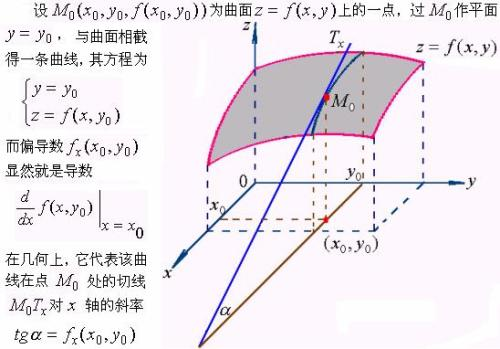
\includegraphics[scale=1.0]{pdsjhyy.jpg}
	
	\subsection{二阶偏导数}
	
	\paragraph{按照对变量的求导顺序不同,二阶偏导数有以下四个}
	1、$\frac{\partial}{\partial x}(\frac{\partial z}{\partial x})=
	\frac{\partial^2z}{\partial x^2}=f_{xx}''(x,y)$\\
	2、$\frac{\partial}{\partial y}(\frac{\partial z}{\partial x})=
	\frac{\partial^2z}{\partial x\partial y}=f_{xy}''(x,y)$\\
	3、$\frac{\partial}{\partial x}(\frac{\partial z}{\partial y})=
	\frac{\partial^2z}{\partial y\partial x}=f_{yx}''(x,y)$\\
	4、$\frac{\partial}{\partial y}(\frac{\partial z}{\partial y})=
	\frac{\partial^2z}{\partial y^2}=f_{yy}''(x,y)$\\
	~\\
	其中$\frac{\partial^2z}{\partial x\partial y}$和$\frac{\partial^2z}{\partial y\partial x}$称为混合偏导数\\
	
	\paragraph{定理}
	若$z=f(x,y)$的两个二阶混合偏导数$\frac{\partial^2z}{\partial x\partial y}$和
	$\frac{\partial^2z}{\partial y\partial x}$在点$(x_0,y_0)$处连续,
	则$\frac{\partial^2z}{\partial x\partial y}|_{(x_0,y_0)}=
	\frac{\partial^2z}{\partial y\partial x}|_{(x_0,y_0)}$\\
	
	\subsection{全微分}
	
	
	
\end{flushleft}
\end{document}